\section{Model description} \label{Model-description}
\subsection{Reactor design}

The Chinese Academy of Sciences proposed the Single-fluid Double-zone Thorium-based Molten Salt Reactor (SD-TMSR) design in 2011
\cite{li_optimization_2018,jiang2012advanced,li2015analysis,li2017model}. The 
\gls{SD-TMSR} is a graphite-moderated molten salt reactor with a thermal power 
of 2,250 MW$_{th}$. The design of the \gls{SD-TMSR} is inspired by the 
\gls{MSBR} \cite{robertson_conceptual_1971} and the \gls{TMSR} 
\cite{nuttin2005potential} after modifying the geometry to control the 
positive moderator temperature coefficient in the MSBR. Li \emph{et al.} and Ashraf \emph{et al.}
described in detail the \gls{SD-TMSR} core geometry
\cite{li_optimization_2018,ashraf2020whole}. The core of the 
\gls{SD-TMSR} is a right cylinder divided into the inner zone (486 fuel tubes) 
and the outer zone (522 fuel tubes) to enhance breeding performance.

In this study, the fuel salt composition is 70LiF - 17.5BeF$_2$ - 
12.5(HM)F$_N$ mole\%, where HM is the heavy metal (i.e. $^{232}$Th and fissile 
materials), and $N$ depends on the chosen fissile material and the 
thermochemical state of the liquid fuel salt. Three different types of initial 
fissile materials are considered: (1) $^{233}$U \cite{ashraf2020whole}, 
(2) reactor-grade Pu \cite{marka1993explosive}, and (3) transuranic (TRU) 
elements from \gls{LWR} \gls{SNF} \cite{de2000scenarios}.
The density and volume of the fuel salt are 3.3 g/cm$^{3}$ and 52.9 m$^3$, 
respectively. The liquid fuel salt circulates continuously through the fuel 
tubes that pierce the graphite hexagonal prisms. The core is surrounded by 
axial and radial graphite reflectors to minimize the neutron leakage.
A 10-cm-thick B$_4$C cylinder surrounds the core to shield against neutrons and heat.
Finally, the \gls{SD-TMSR} pressure vessel holds all reactor components and is made of 
a Hastelloy N alloy. The main characteristics of the \gls{SD-TMSR} are 
summarized in Table~\ref{tab:table1}.


\begin{table}  %[!ht]
	\caption{The main characteristics of the SD-TMSR \cite{li_optimization_2018,ashraf2020whole}.}
	\vspace{0.1in}
	\begin{tabularx}{\textwidth}{l | r}
		\hline
		Thermal power, MW$_{th}$          				&  2,250  \\ 
		Fuel salt components                            & LiF-BeF$_2$-(\gls{HM})F$_N$ \\
		Fuel composition, mole\%                        & 70-17.5-12.5    \\
		$^7$Li enrichment, \%        				& 99.995   \\
		Fuel temperature, K 							& 900  \\
		Fuel density at 900 K, g/cm$^3$		  		& 3.3 \\
		Fuel dilatation coefficient, g/(cm$^3$$.$K)  &  -6.7$\times$10$^{-4}$ \\
		Graphite density, g/cm$^3$             	    & 2.3	\\ 
		B$_4$C density, g/cm$^3$					& 2.52  \\ 
		Core diameter, cm								& 460  \\
		Core height, cm									& 460  \\
		Side length of the graphite hexagonal prism, cm   & 7.5 \\
		Inner radius, cm							& 3.5  \\
		Outer radius, cm							& 5  \\
		Ratio of molten salt and graphite in the inner zone	&  0.357  \\
		Ratio of molten salt and graphite in the outer zone &  1.162  \\
		Fuel volume, m$^3$  &	52.9 \\
		\hline
	\end{tabularx}
	\label{tab:table1}
\end{table}
%%%%%%%%%%%%%%%%%%%%%%%%%%%%%%%%%%%%%%%%


\subsection{Control rod design} \label{CRD}

The reactivity of the SD-TMSR core is controlled by two clusters of control 
rods:
\begin{enumerate}
\item Control Safety Devices (CSD);
\item Shutdown Safety Devices (SSD).
\end{enumerate}
The CSD system is designed for reactivity control during normal operation and the SSD system is designed for an emergency reactor shutdown.
In the present work, six different absorbing materials are considered based on their neutronics and safety performance:
\begin{enumerate}
\item natural B$_4$C (19.9\% $^{10}$B);
\item B$_4$C with boron enriched to 90\% $^{10}$B;
\item hafnium diboride (HfB$_2$);
\item hafnium hydride (HfH$_{1.62}$);
\item gadolinium oxide (Gd$_2$O$_3$);
\item europium oxide (Eu$_2$O$_3$).
\end{enumerate}

The control rod is a cylinder with a radius of 0.75 cm and a height of 520 cm. 
The absorbing material is surrounded by a 0.25-cm-thick cladding made of AIM1 
(15Cr-15Ni) steel alloy \cite{SERAN2017285} and the guide tube is made of 
SiC structural material (see Figure~\ref{fig:cr}). We simulated a small gap between the 
cladding and guide tube to facilitate the control rod movement.

Since the total number and distribution of the control assemblies in the SD-TMSR are unknown, we proposed an original distribution as a starting point of this analysis. We added clusters consist of four control rods to specific graphite hexagonal prisms (elements) in the SD-TMSR core. Every four control rods (cluster) can move together as one group. Figure~\ref{fig:graphite_elemen} and~\ref{fig:graphite_elemen1} demonstrate the plan and axial view of the graphite element with the control rods. The total number of graphite elements with control rods are 25: 16 CSD and 9 SSD.
\begin{figure}[t!]  % replace 't' with 'b' to \centering
	\centering
	\hspace{+0.65in} 
	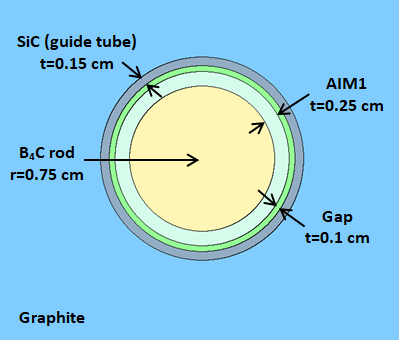
\includegraphics[width=\textwidth]{cr.png}
	\caption{Cross section of the B$_4$C control rod.}
	\label{fig:cr}
\end{figure}
\begin{figure}[t!]  % replace 't' with 'b' to \centering
	\centering
	\hspace{+0.65in}
	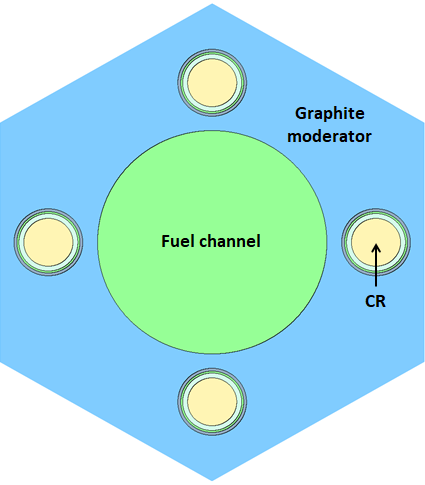
\includegraphics[width=\textwidth]{graphite_element.png}
	\caption{$XY$ section of graphite element with the four control rods 
	(cluster) located at the same distance from the fuel channel.}
	\label{fig:graphite_elemen}
\end{figure}
\begin{figure}[t!]  % replace 't' with 'b' to \centering
	\centering
	\hspace{+0.65in}
	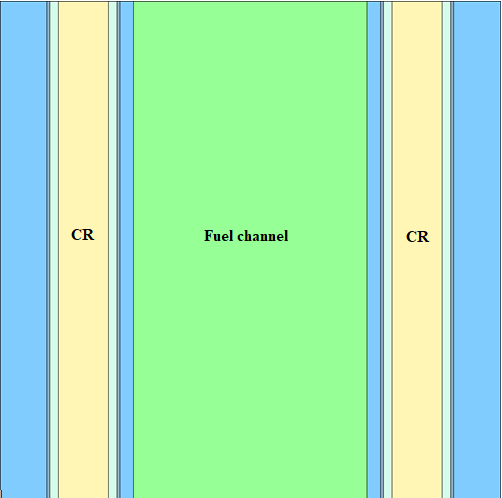
\includegraphics[width=\textwidth]{graphite_element1.png}
	\caption{$XZ$ section of graphite element with control rods.}
	\label{fig:graphite_elemen1}
\end{figure}

Figure~\ref{fig:core_25} illustrates the numbering scheme of control rods 
clusters in the SD-TMSR core.
The CSD1-16 clusters are represented as yellow color and distributed as two rings: inner and outer ring (peripheral ring). The inner ring includes CSD from 1 to 6, while the outer ring includes CSD from 7 to 16. Red color stands for SSD1-9 clusters.
We distributed the graphite elements with control rods clusters uniformly in 
the inner core of the SD-TMSR, in which the moderator-to-fuel ratio is high.
The selected core segment at the upper left corner of the 
Figure~\ref{fig:core_25} shows that both CSD and SSD clusters consist of four 
control rods located at the same distance from the fuel channel center.
\begin{figure}[t!]  % replace 't' with 'b' to \centering
	\centering
	\hspace{+0.65in}
	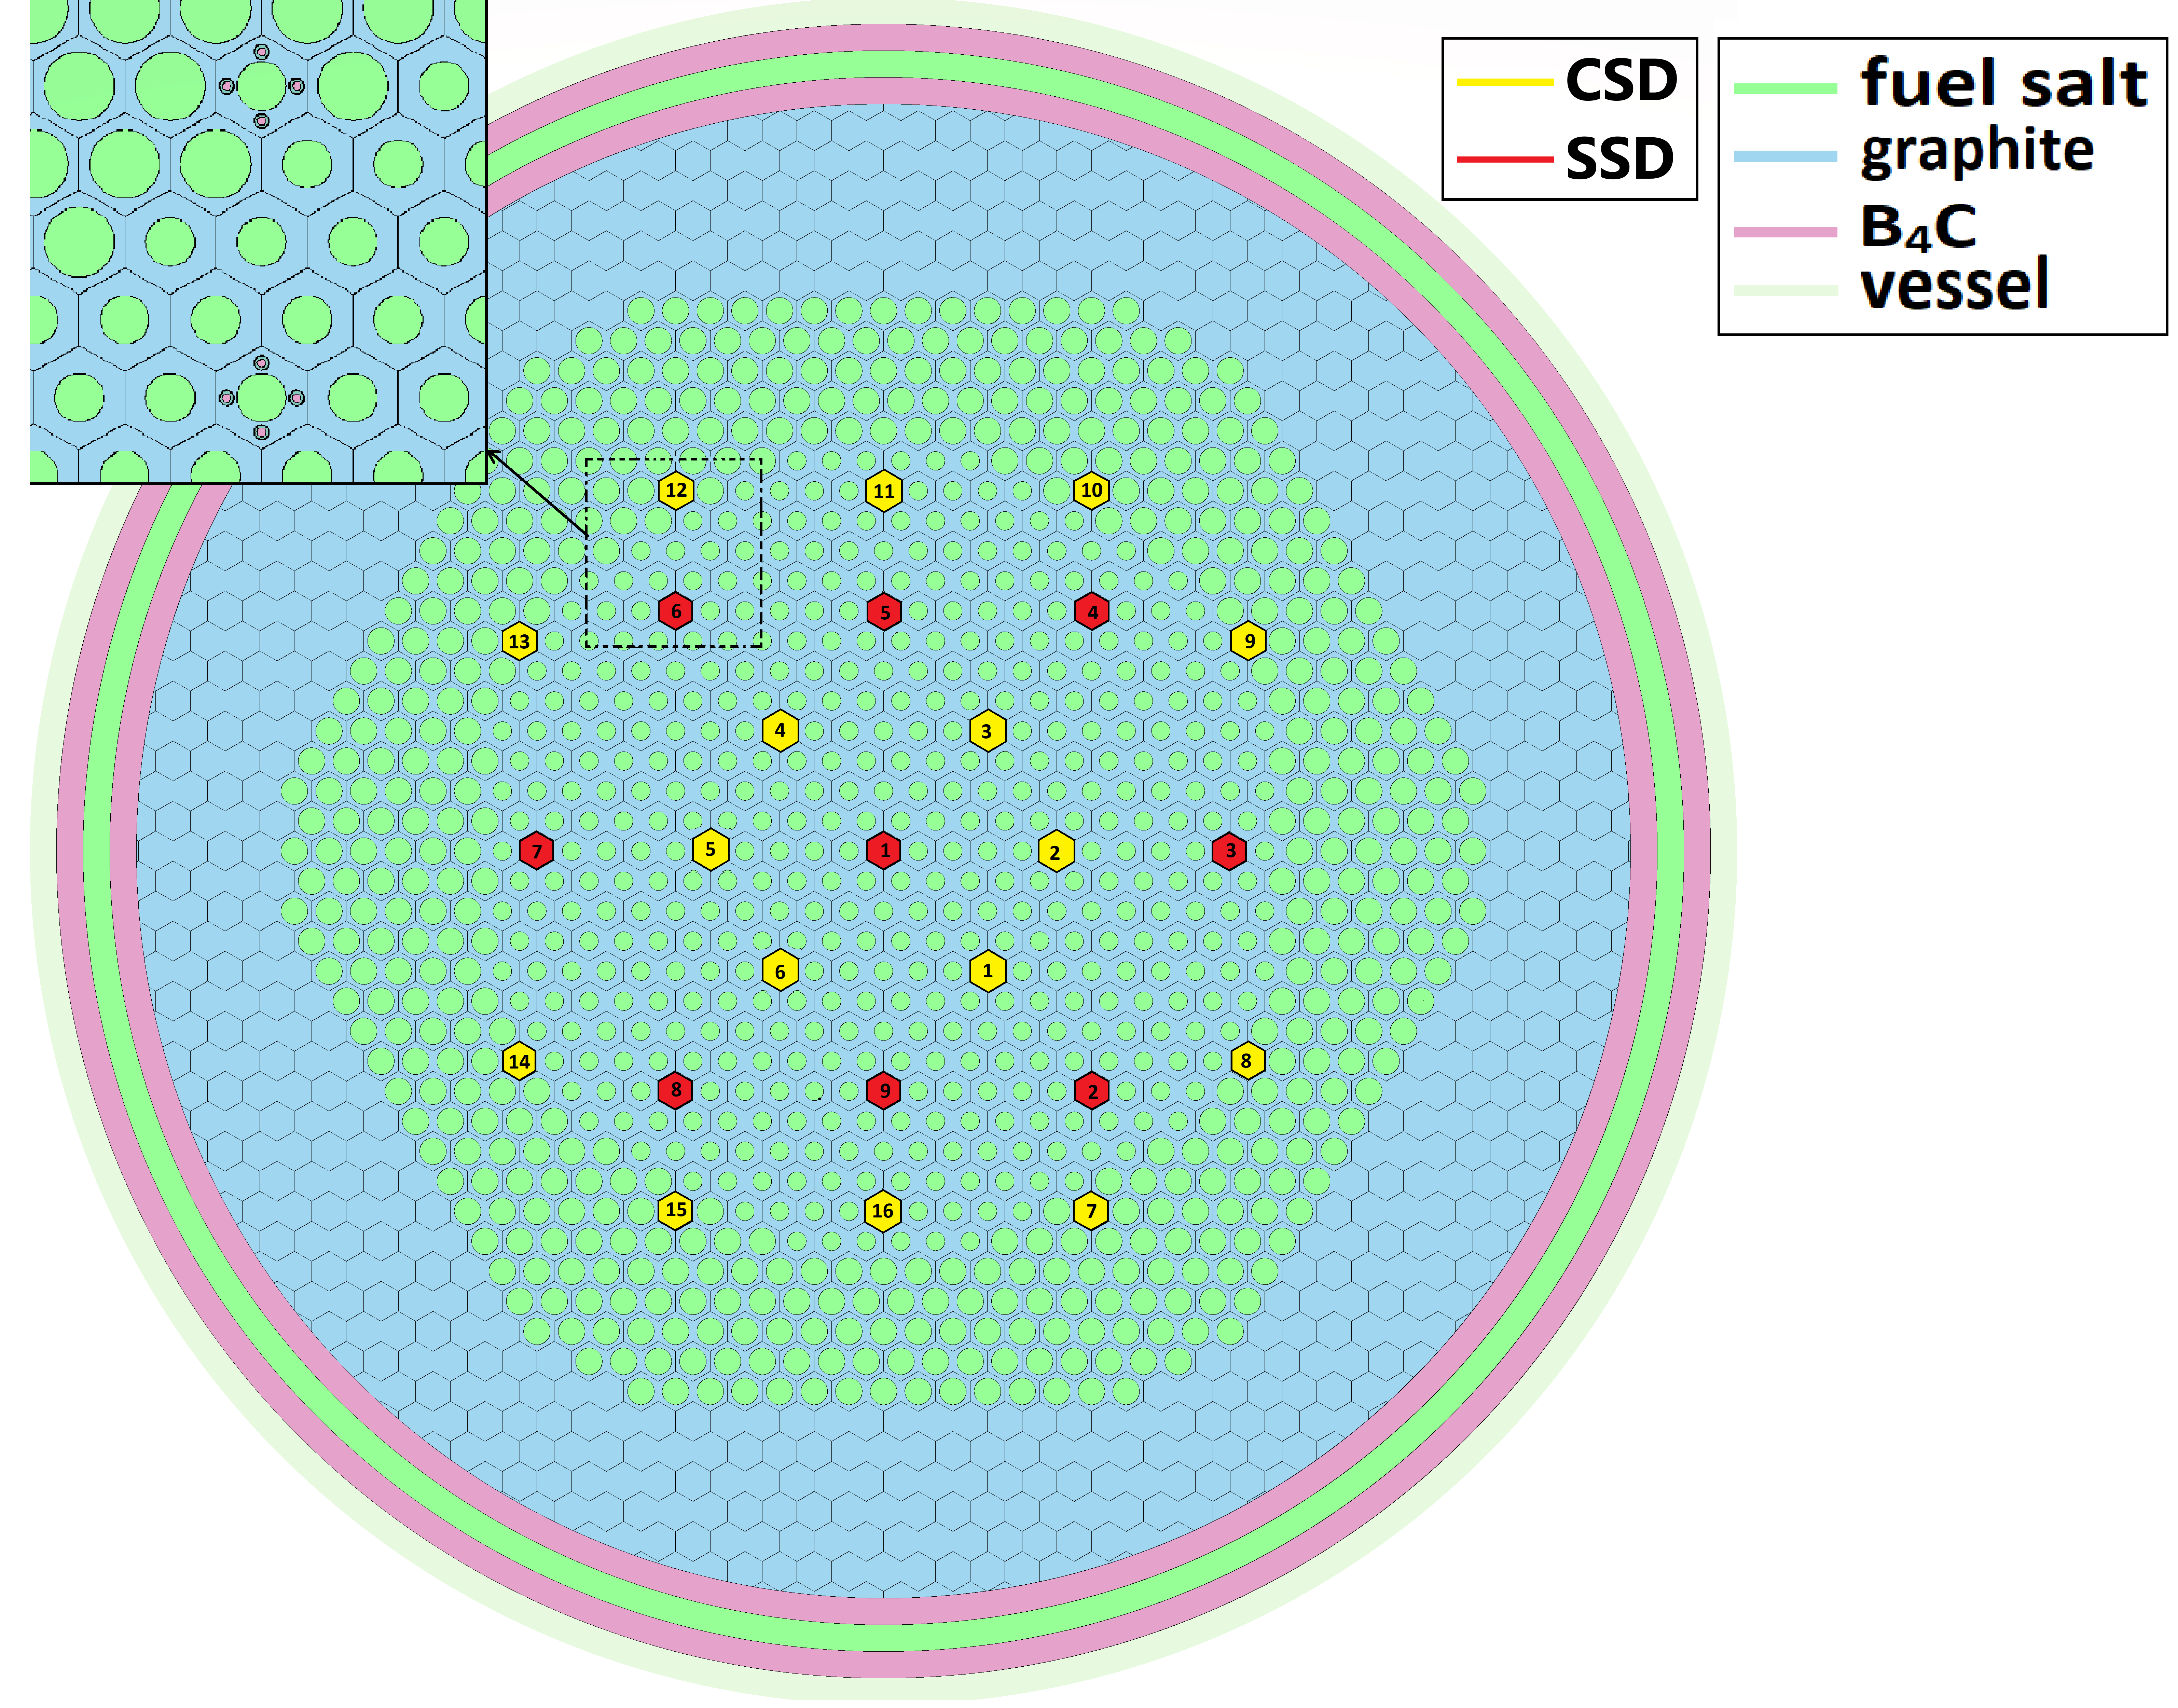
\includegraphics[width=\textwidth]{core_25.png}
	\caption{Distribution of the graphite elements with control rods in the SD-TMSR core. Green - fuel salt, blue - graphite, pink - B$_4$C, and light-green - vessel (H-alloy).}
	\label{fig:core_25}
\end{figure}

\section{Methodology and tools} \label{Methodology-and-tools}
\subsection{Control rod design evaluation}
In this work, SERPENT-2 \cite{leppanen2014serpent} is used to 
perform steady state calculations for the full-core of the SD-TMSR with 
suggested control rod design. We adopted the ENDF-VII.0 cross section library 
for all calculations in the present work. The results demonstrate whole-core 
runs of $50,000$ neutrons per cycle, for 50 inactive and 500 active cycles. The 
statistical error in $k_{eff}$ from SERPENT-2 output is $\leq$ $25$ 
$pcm$.

The initial calculation state of the SD-TMSR is identified by normal operation 
conditions (see Table~\ref{tab:table1}) and fully withdrawn control rods 
clusters. In this case, the control rods are located above the upper plenum as 
shown in Figure~\ref{fig:core_26}. To validate the proposed control rods 
system we adopted the same operation conditions (as in the initial calculation 
state) and changed the position of the control rod clusters along $Z$ 
direction. The main calculated parameters including reactivity, control rod 
worth, and interference effects (shadowing effects) are described below.

\begin{figure}[t!] % replace 't' with 'b' to \centering
	\centering
	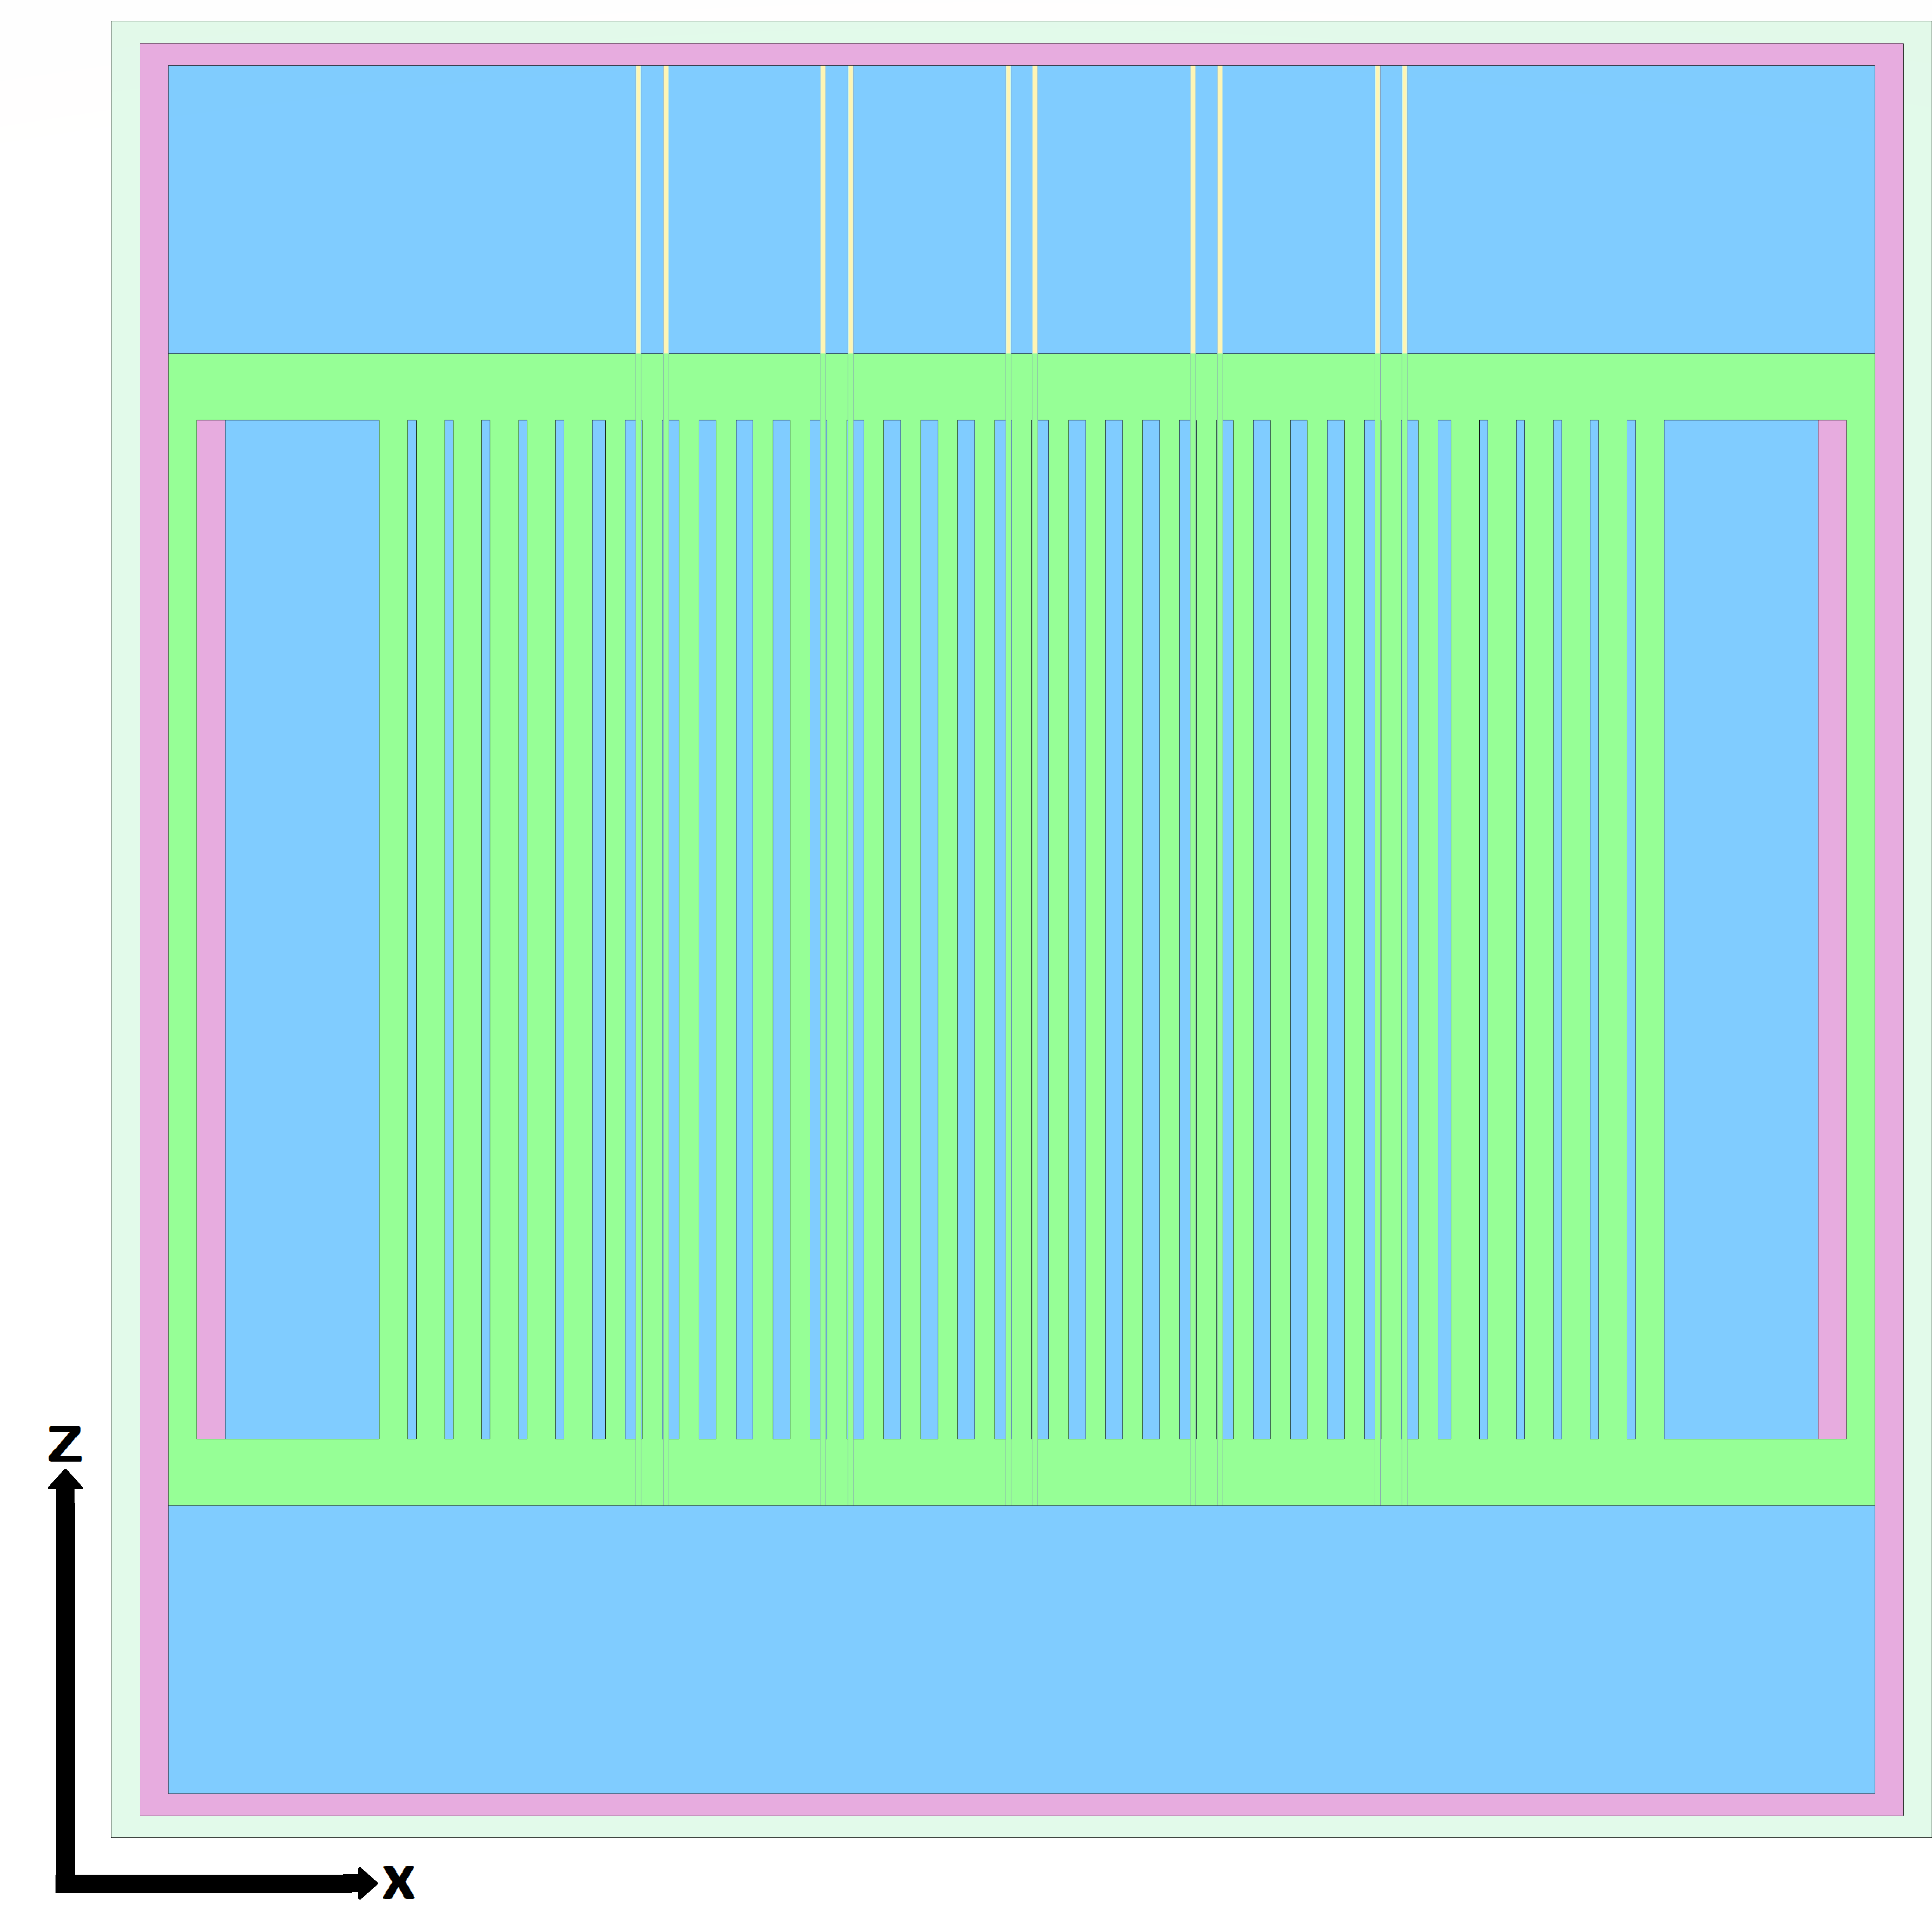
\includegraphics[width=\textwidth]{core_26.png}
	\caption{$XZ$ view at the midplane of the full-core model of the SD-TMSR, 10 CRs are fully withdrawn.}
	\label{fig:core_26}
\end{figure}

\subsubsection{Reactivity calculation}

The excess reactivity $\rho$$_e$ is the reactivity of the core when all control rods are withdrawn. $\rho$$_e$ is calculated by SERPENT-2 in \$ units based on equation~\ref{Equ:1}, where $k_{eff}$ is the effective multiplication factor of the core and $\beta_{eff}$ is the effective fraction of delayed neutrons. The effective delayed neutron fraction is calculated by the adjoint-weighted time constants using perturbation technique in SERPENT-2 \cite{leppanen2014calculation}.

\begin{equation}
\label{Equ:1}
{{\rho}_{e}}=\dfrac{{k_{eff}}-1}{{k_{eff}}{{\beta}_{eff}}},
\end{equation}

\subsubsection{The control rod worths (CRW)}

The control rod worth (CRW) is the amount of negative reactivity that associated with the control rod insertion. The CRW is calculated by SERPENT-2 in \$ units based on equation~\ref{Equ:2}, where $\Delta\rho$$_{CRi}$ is the worth of i$^{th}$ CR, $\rho$$_e$ is the initial excess reactivity, and $\rho$$_{CRi}$ is the excess reactivity after insertion i$^{th}$ CR \cite{vcerba2017optimization}.

\begin{equation}
\label{Equ:2}
{{\Delta}{\rho}_{CRi}}={{\rho}_{e}}-{{\rho}_{CRi}},
\end{equation}

\subsubsection{Shutdown Margin (SDM)}

The shutdown margin (SDM) is the amount of reactivity by which a full reactor core is subcritical from a given state. The SDM is expressed in terms of reactivity and calculated by equation~\ref{Equ:6}, where $\Delta\rho_{SSD}$ is the total worth of the Shutdown Safety Devices (SSD) and $\rho$$_e$ is the core excess reactivity.

\begin{equation}
\label{Equ:6}
{SDM}={{\Delta}{\rho}_{SSD}}-{{\rho}_{e}},
\end{equation}

\subsubsection{Interference effects (shadowing effects)}

Interference between control rods (CRs) or shadowing effects occur when one 
(or more) control rod affects the reactivity worth of another control rod in 
the surroundings. Thus, the shadowing effect appears when the combined rod worth
is less than the sum of the individual worths. Oppositely, anti-shadowing is observed 
when the combined rod worth is greater than the sum of the individual worths.
The core height-to-diameter ratio (H/D) and the three-dimensional configuration 
of the control rods affect the degree of the interference between CRs \cite{girardin2007control}. 

The amplification factor (A$_{CRi}$) of i$^{th}$ control rod helps to evaluate the shadowing effects between control rod clusters. The amplification factor is calculated by equation~\ref{Equ:3} \cite{girardin2007control,vcerba2017optimization}, where $\Delta\rho$$_{CR(1,2,\ldots N)}$ is the total worth of all control rods (from $1$ to $N$), $\Delta\rho$$_{CR(1,2,\ldots N-i)}$ is the total worth of all CRs except the investigated one i$^{th}$ and $\Delta\rho$$_{CRi}$ the worth of the i$^{th}$ rod.

\begin{equation}
\label{Equ:3}
{{A}_{CRi}}=\dfrac{{{\Delta}{\rho}_{CR(1,2,\ldots N)}}-{{\Delta}{\rho}_{CR(1,2,\ldots N-i)}}}{{\Delta}{\rho}_{CRi}},
\end{equation}

If A$_{CRi}$ is $<$1, the control rod worth is reduced due to shadowing effects, while if A$_{CRi}$ is $>$1 the control rod worth is amplified and anti-shadowing effects occur. A$_{CRi}$ = 1 means no shadowing effects occur.

\subsubsection{Integral and differential control rod worth}

The integral CRW is the total reactivity change due to the control rod full 
insertion or withdrawal. However, the differential CRW is the amount of 
reactivity inserted per unit of withdrawal [\$/cm]. To calculate those 
parameters, we varied the position of CRs clusters from fully withdrawn to 
fully inserted. Equation~\ref{Equ:4} is used to calculate the integral CRW 
[\$], where $k_{j}$ and $k_{j-1}$ are the effective multiplication factor 
after and before CR insertion to $j$$^{th}$ step. $\beta_{j}$ is the effective 
fraction of delayed neutrons at $j$$^{th}$ step. $N$ is the number of steps.

\begin{equation}
\label{Equ:4}
{{\Delta}{\rho}_{j}}=\sum_{j=1}^{N}\dfrac{{k_{j}}-{k_{j-1}}}{{{k_{j}}{k_{j-1}}}{{\beta}_{j}}},
\end{equation}

Equation~\ref{Equ:5} is used to calculate the differential CRW [\$/cm], where 
$Z$ is the coordinate of the bottom of the control rod.

\begin{equation}
\label{Equ:5}
\dfrac{{\partial}{\rho}_{j}}{{\partial{Z}}}=\dfrac{1}{{\Delta}{Z}}\dfrac{{k_{j}}-{k_{j-1}}}{{{k_{j}}{k_{j-1}}}{{\beta}_{j}}},
\end{equation}


